\chapter*{My Own Data Mining}
\stepcounter{chapter}

\section*{}
\paragraph{Hypothesis:} \textbf{In Biden-voting states, income is more strongly correlated with education level, whereas in
Trump-voting states, income is more strongly correlated with 'hours worked'}
\textit{Prove or disprove if there is evidence to suggest the wealth in the Democratic states is knowledge orientated (more white collar work),
whereas in then states where Trump had more residence, the wealth was found in more blue collar workers.} 

\subsection{Underlying Trends}
\begin{figure}[H]
     \centering
     \begin{subfigure}[b]{0.45\textwidth}
         \centering
         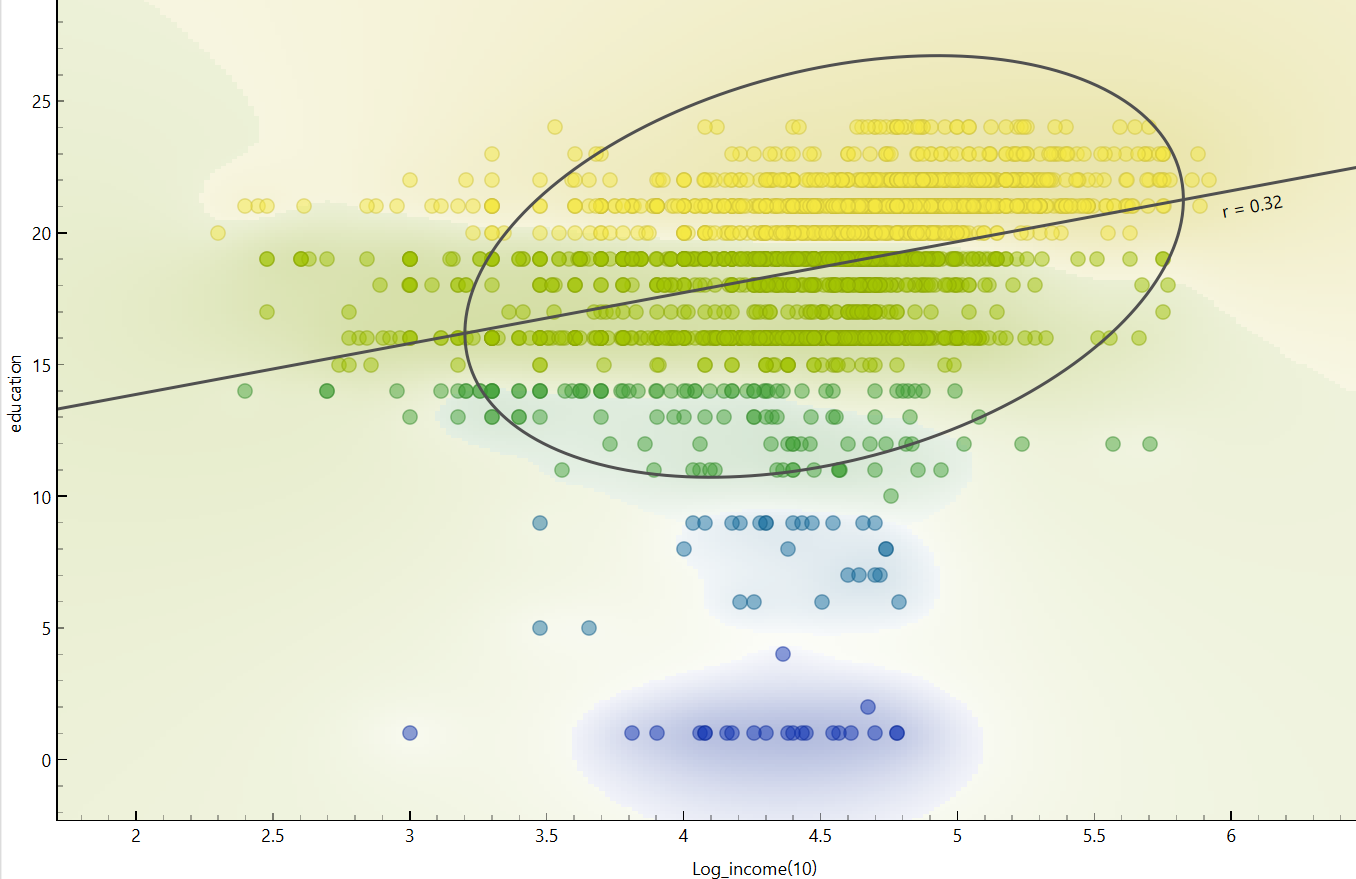
\includegraphics[width=\textwidth]{chapters/part 5 - images/Biden_edu_vs_log(inc).png}
         \caption{Democrat voters education level vs their income.}
         \label{fig:Biden_education_states}
     \end{subfigure}
     \hfill
     \begin{subfigure}[b]{0.45\textwidth}
         \centering
         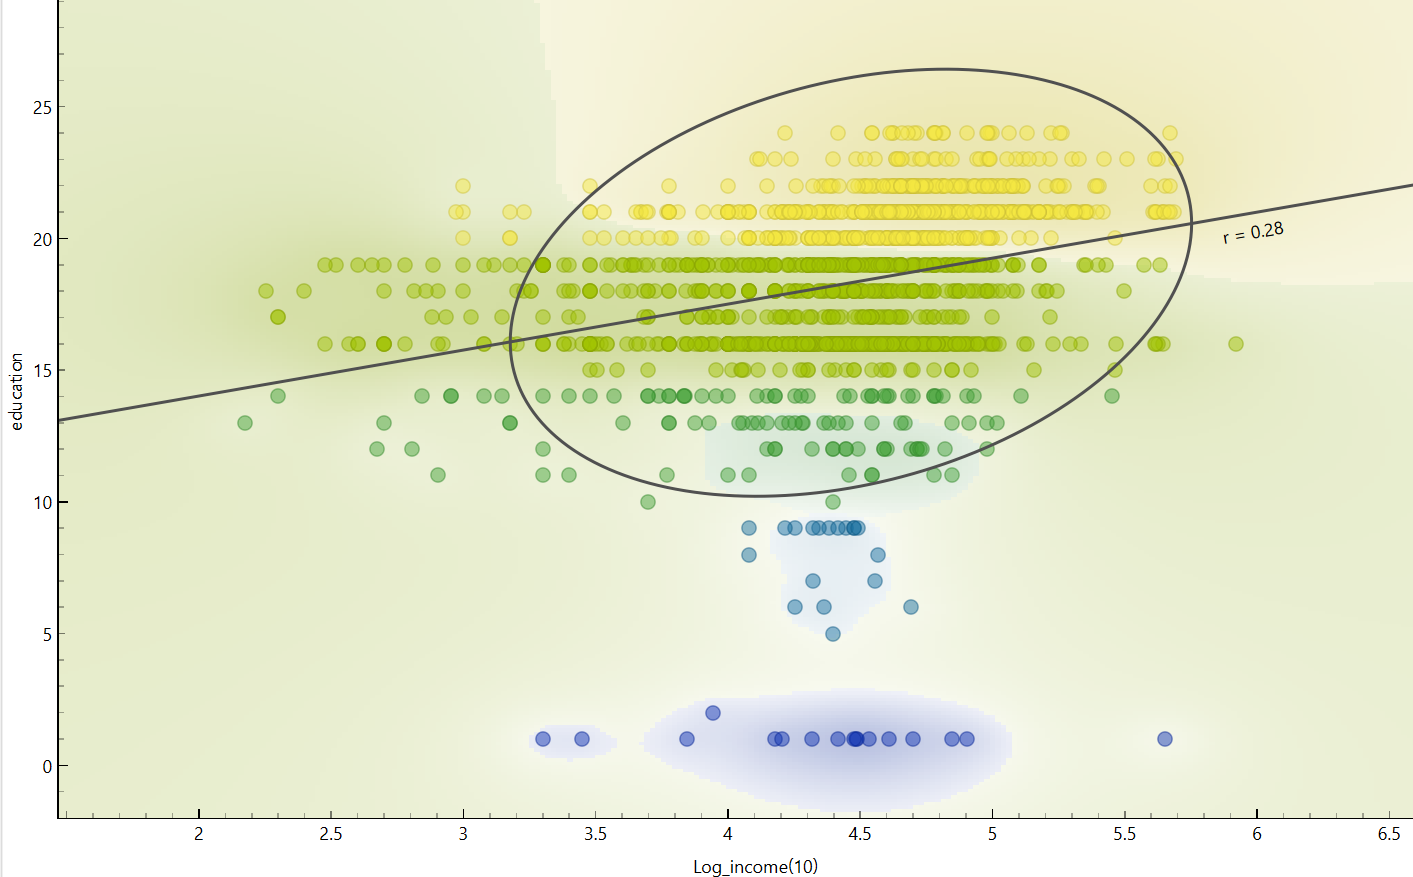
\includegraphics[width=\textwidth]{chapters/part 5 - images/Trump_edu_vs_log(inc).png}
         \caption{Republican voters education level vs their income.}
         \label{fig:Trump_education_states}
     \end{subfigure}
     \caption{Education vs Income in each subgroup of voters split by state winning party.}
     \label{fig:edu_vote_distribution}
\end{figure}
As previously discussed, there is a greater correlation between the Education level and Income in states which voted more for Biden,
with $r=0.32 > p=0.28$. This helps to identify that in Biden voting states, Education relates more to their income, compared to those
that voted Trump.

To further illustrate this point, the department/type of job that people get their income from will be checked.
\begin{figure}[H]
     \centering
     \begin{subfigure}[b]{0.45\textwidth}
         \centering
         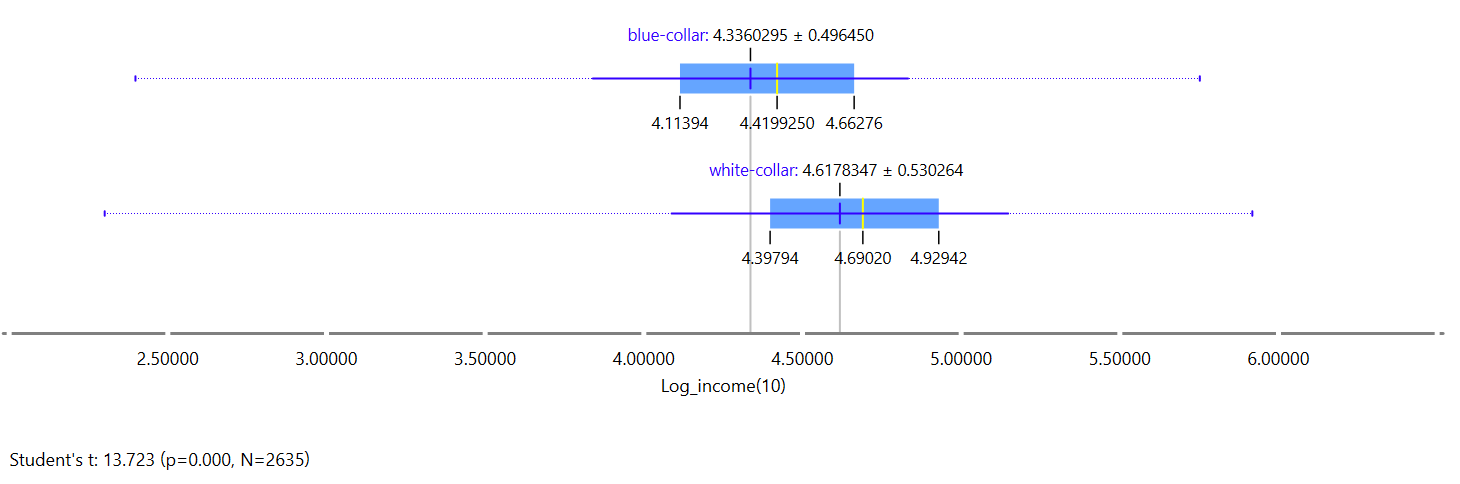
\includegraphics[width=\textwidth]{chapters/part 5 - images/Biden_income_collar.png}
         \caption{Democrat voter job spread.}
         \label{fig:Biden_collar}
     \end{subfigure}
     \hfill
     \begin{subfigure}[b]{0.45\textwidth}
         \centering
         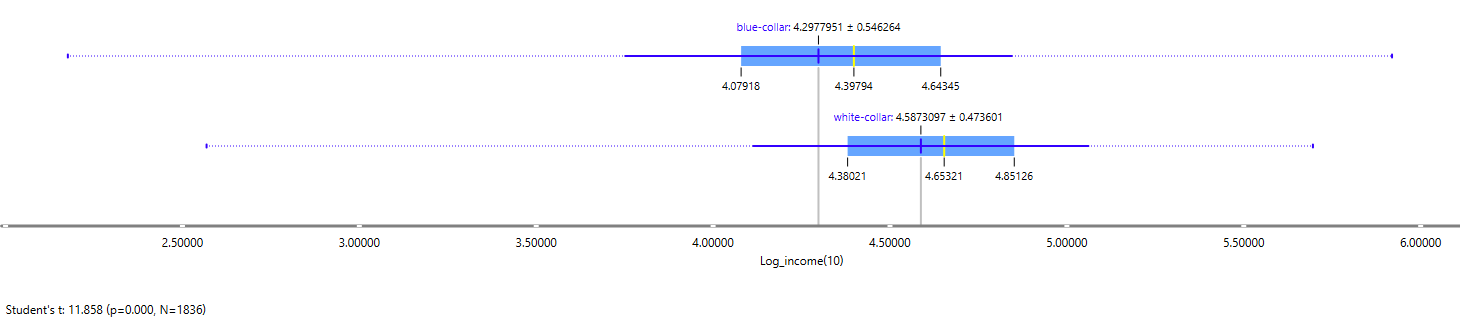
\includegraphics[width=\textwidth]{chapters/part 5 - images/Trump_income_collar.png}
         \caption{Republican voter job spread.}
         \label{fig:Trump_collar}
     \end{subfigure}
     \caption{How are Blue and White Collar jobs distributed.}
     \label{fig:voter_collar_distribution}
\end{figure}
While the income for '\texttt{White Collar}' jobs (requiring greater Education levels) remain the greatest across all states, those in Biden voting states appear to
earn $\approx\$2,000$ more. With the White-collar distribution in Biden states having a higher mean income, compared to those in
Trump voting states. However, with wider whiskers in Biden states, it suggests that there is a greater degree of income inequality
compared to those in Trump biased states, where it shows a more middle-class distribution.

\subsection{Predictive Voting}
\subsubsection{Limitations}
Since voting statistics are state wide distributions and do not correlate to specific individuals, it is harder to determine
who someone will vote for simply based on proxy labelling. However, models may be formed on underlying patterns which (despite
lack of expected accuracy) hint towards more trends within the data.

\subsubsection{Model Prediction}
\begin{figure}[H]
    \centering
    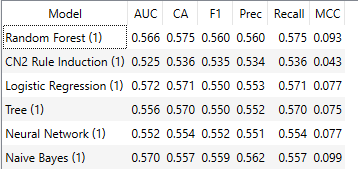
\includegraphics[width=0.7\textwidth]{chapters/part 5 - images/Predicability.png}
    \caption{Varying model predictability.}
\end{figure}
\textbf{Random Forest} is the most accurate despite being only slightly better than a guess. This failure is also shown by the 
\texttt{Matthews Correlation Coefficient (MCC)} which measures how good models are for binary classifications (\texttt{Trump, Biden}). With all
models $MCC<0.1$ they are all very bad at determining the correct class.

While the models are weak and don't predict who someone votes for very accurately (likely due to the vast range of individuals
within the sub-set who did not vote for Biden or Trump respectively but were classified as such); the model can be used
to help suggest trends within the data that point to an overall classification.
\begin{figure}[H]
     \centering
     \begin{subfigure}[b]{0.45\textwidth}
         \centering
         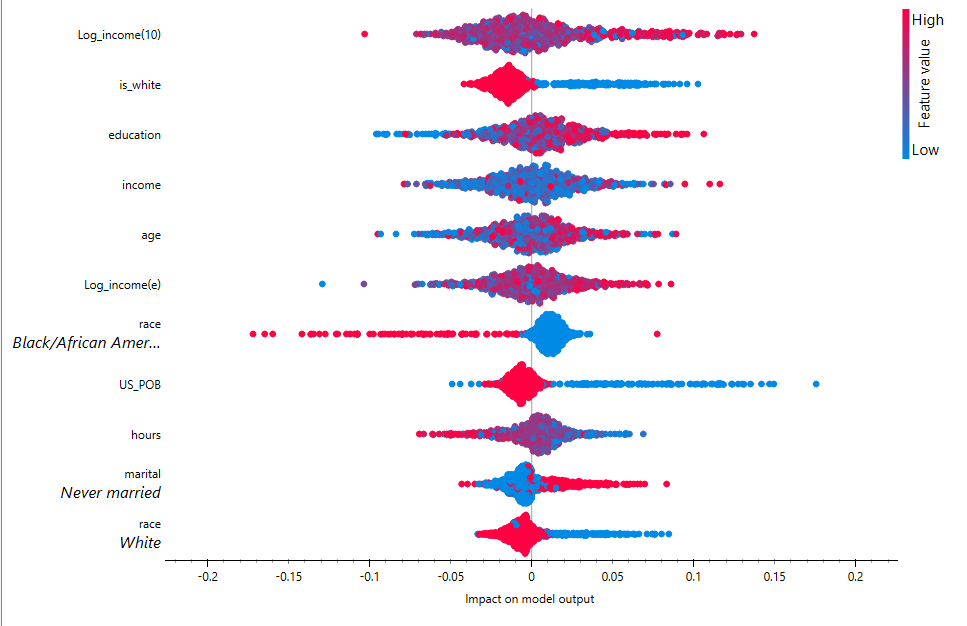
\includegraphics[width=0.7\textwidth]{chapters/part 5 - images/model_influences.png}
         \caption{Standout variables that effect the prediction.}
         \label{fig:pred_influences}
     \end{subfigure}
     \hfill
     \begin{subfigure}[b]{0.45\textwidth}
         \centering
         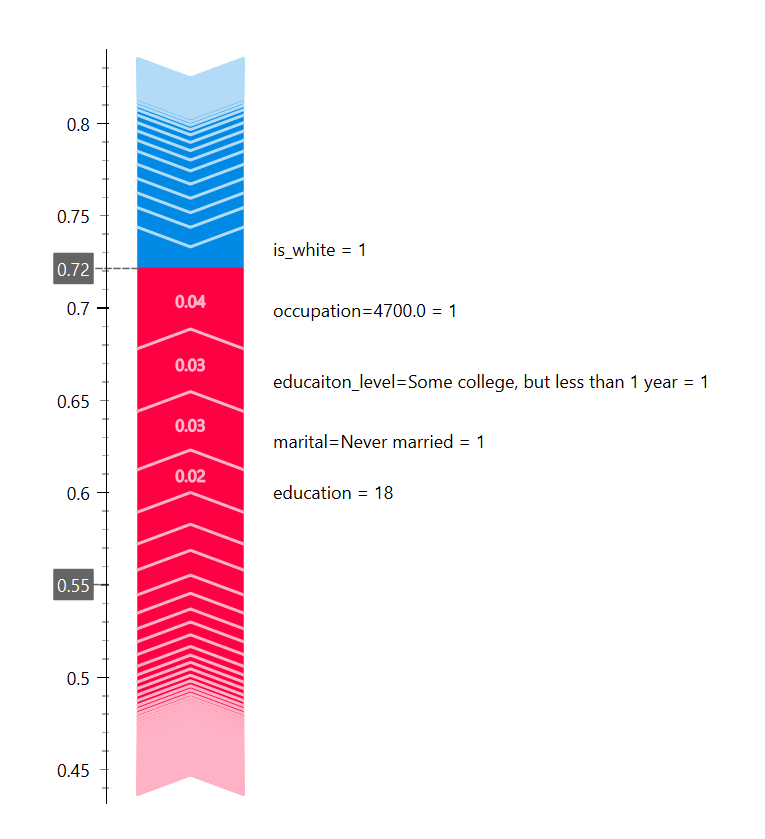
\includegraphics[width=\textwidth]{chapters/part 5 - images/model_SHAP_Biden.png}
         \caption{Specific variable instance bias.}
         \label{fig:Biden_pred_influences}
     \end{subfigure}
     \caption{How variables affect the voting prediction.}
     \label{fig:pred_voting}
\end{figure}
Figure \ref{fig:pred_influences} shows how varying values influence the models prediction towards someone voting for Biden,
with factors such as:
\begin{itemize}
    \item \textbf{Higher income} levels correlate with a stronger prediction for Biden.
    \item Identifying as \textbf{white} acts as a negative predictor for Biden, pushing the classification toward Trump.
    \item Specific \textbf{occupation codes} (such as 4700, representing Retail/Service roles) contribute positively to a Biden prediction.
    \item Being \textbf{never married} or single increases the probability of a Biden vote, aligning with more liberal urban demographics.
    \item Educational exposure, specifically \textbf{starting but not completing college}, is shown to increase the likelihood of a Biden
    prediction.
\end{itemize}


\subsection{Are there any racial factors that effect voting habits?}
Following the identification of \textbf{Race} on voting patterns, what is the variation between the candidates.
\begin{figure}[H]
     \centering
     \begin{subfigure}[b]{0.45\textwidth}
         \centering
         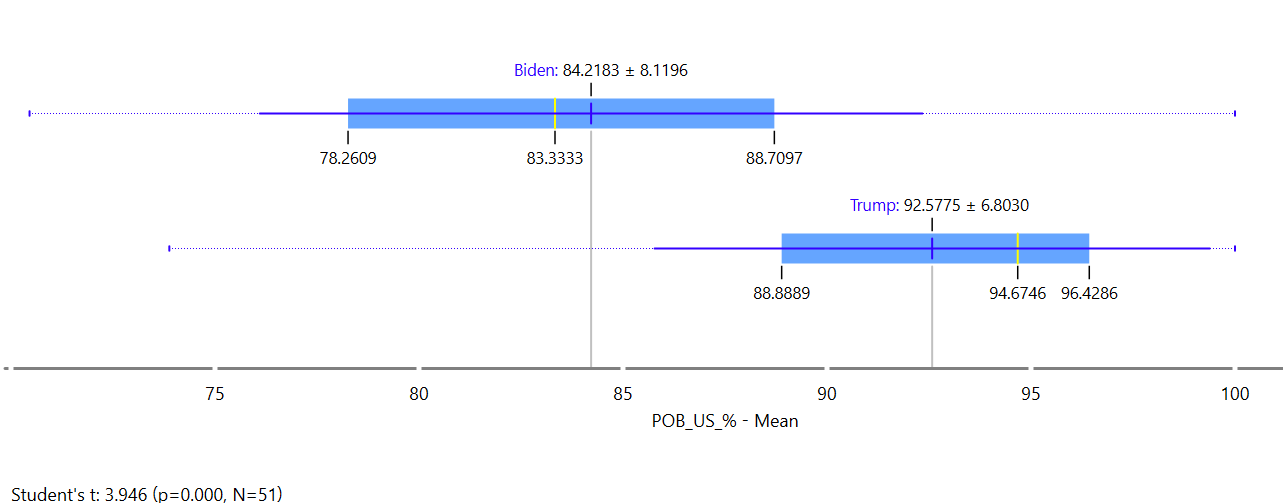
\includegraphics[width=0.7\textwidth]{chapters/part 5 - images/POB_perc.png}
         \caption{Proportions of voters \textbf{born in the US} for each Candidate.}
         \label{fig:POW perc}
     \end{subfigure}
     \hfill
     \begin{subfigure}[b]{0.45\textwidth}
         \centering
         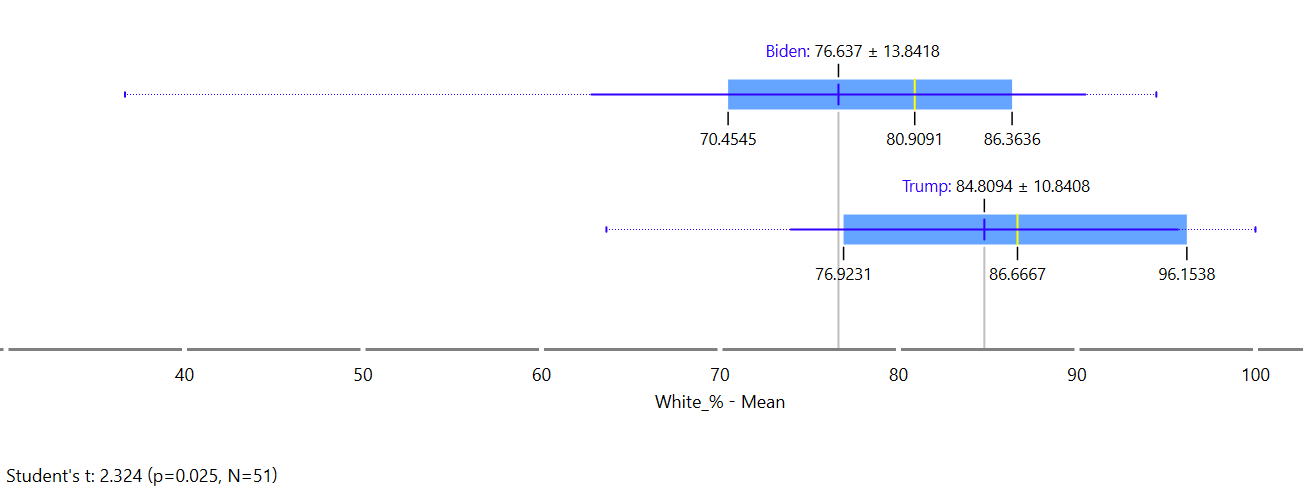
\includegraphics[width=\textwidth]{chapters/part 5 - images/White_perc.png}
         \caption{Proportions of voters who are \textbf{White} for each Candidate.}
         \label{fig:WHITE perc}
     \end{subfigure}
     \caption{Race and Background of each candidate's voters.}
     \label{fig:Voter Background}
\end{figure}
With $P=0.000 and P=0.025$ respectively ($<0.05$), there is sufficient evidence to suggest that Trump-voting states ($\approx84.8\%$) have a higher proportion of
\texttt{white} voters than Biden-voting states ($\approx76.6\%$) as well as Biden-voting states containing a significantly higher proportion of voters born
\texttt{outside the US}.

\section{Summary}
In summary, predicting individual voting behaviour is not feasible from the data provided; however, features such as \textbf{Place of Birth}, \textbf{White or not},
and \textbf{Industry} can all help point towards a preference for one candidate over another. Conversely, for specific categories such as shipping office
workers or widowed individuals, there is a lack of cases to support a clear classification. This essentially adds noise to the data. In this instance, utilising a
larger sample size or individual-level voting records would allow for a more accurate model that can identify patterns more easily.

\begin{figure}[H]
    \centering
    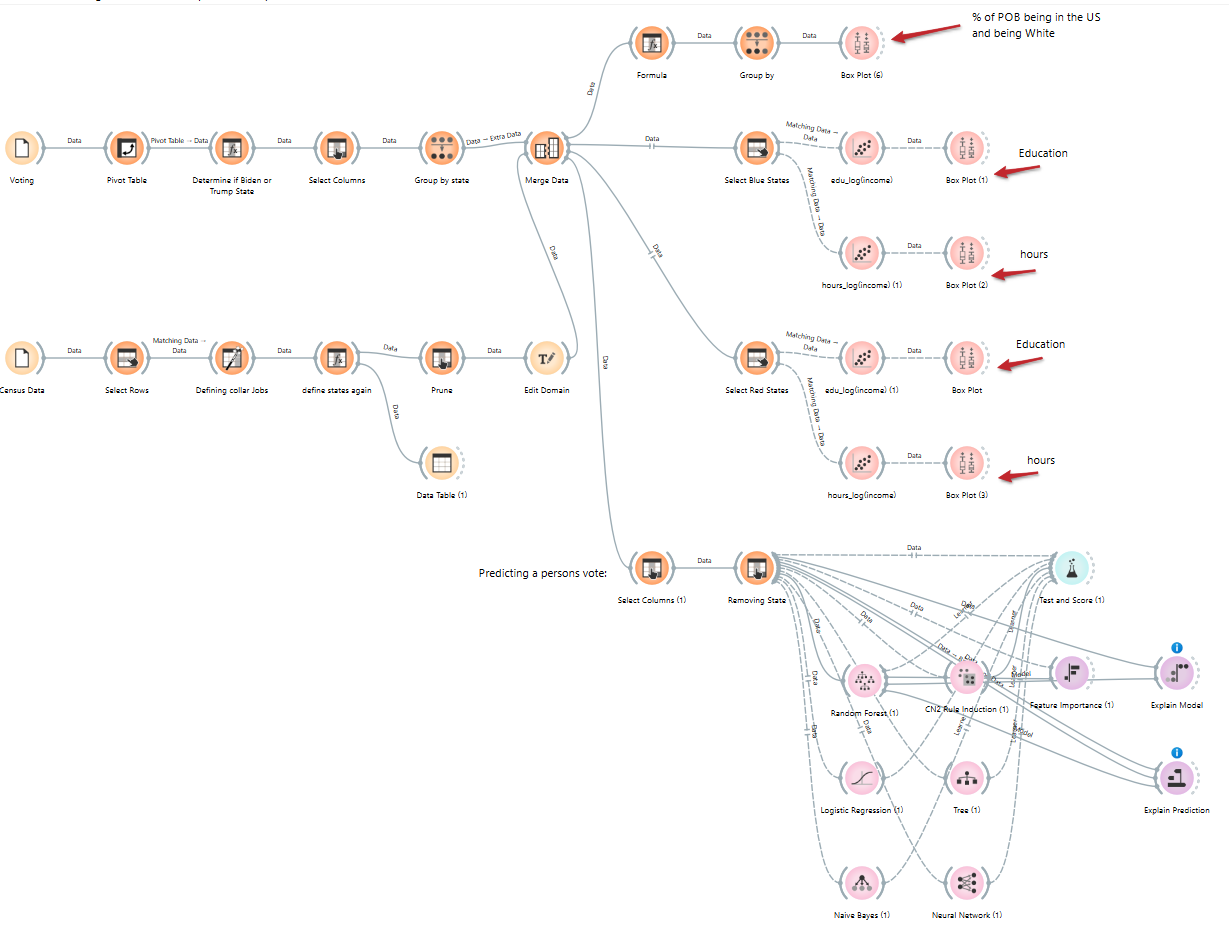
\includegraphics[width=\textwidth]{chapters/part 5 - images/node_structure.png}
    \caption{My Data mining Structure.}
    \label{fig:my_data_mining}
\end{figure}